% !TeX root = main.tex
\documentclass{article} % Or report, book, etc.
\usepackage{graphicx}  % Required for \includegraphics
\usepackage{amsmath}   % Required for math symbols like \pi

\begin{document}

% Define performance metrics before the figure
We evaluate the performance on the Cloth Folding task using two metrics. First, the raw performance \(P\) is calculated based on the particle positions:
\begin{equation} \label{eq:performance}
P = - \left( \frac{1}{M} \sum_{i \in G_a} \| \mathbf{p}_i - \mathbf{p}_{j(i)} \|_2 \right) - 1.2 \times \left( \frac{1}{M} \sum_{j \in G_b} \| \mathbf{p}_j - \mathbf{p}_{j, init} \|_2 \right)
\end{equation}
where \(M\) is the number of particles per fold group, \(G_a, G_b\) are the particle sets for the two halves being folded together, \(\mathbf{p}_i\) is the current 3D position of particle \(i\), \(\mathbf{p}_{j(i)}\) is the current 3D position of the corresponding particle in the other group, and \(\mathbf{p}_{j, init}\) is the initial 3D position of particle \(j\) in the fixed group.
This raw performance is then normalized to a scale, representing the progress from the initial state towards an ideal fold. The ideal performance \(P_{ideal} = 0\) occurs when corresponding particles align (\(\| \mathbf{p}_i - \mathbf{p}_{j(i)} \|_2 \to 0\)) and fixed particles remain stationary (\(\| \mathbf{p}_j - \mathbf{p}_{j, init} \|_2 \to 0\)), causing both terms in Equation~\eqref{eq:performance} to vanish. The normalized performance is:
\begin{equation} \label{eq:norm_performance}
P_{\text{norm}} = \frac{P - P_{init}}{P_{ideal} - P_{init}} = \frac{P - P_{init}}{- P_{init}}
\end{equation}
where \(P_{init}\) is the raw performance calculated using Equation~\eqref{eq:performance} at the start of the episode.

\begin{figure}[htbp] % Use [htbp] for placement preference: here, top, bottom, page
    \centering
    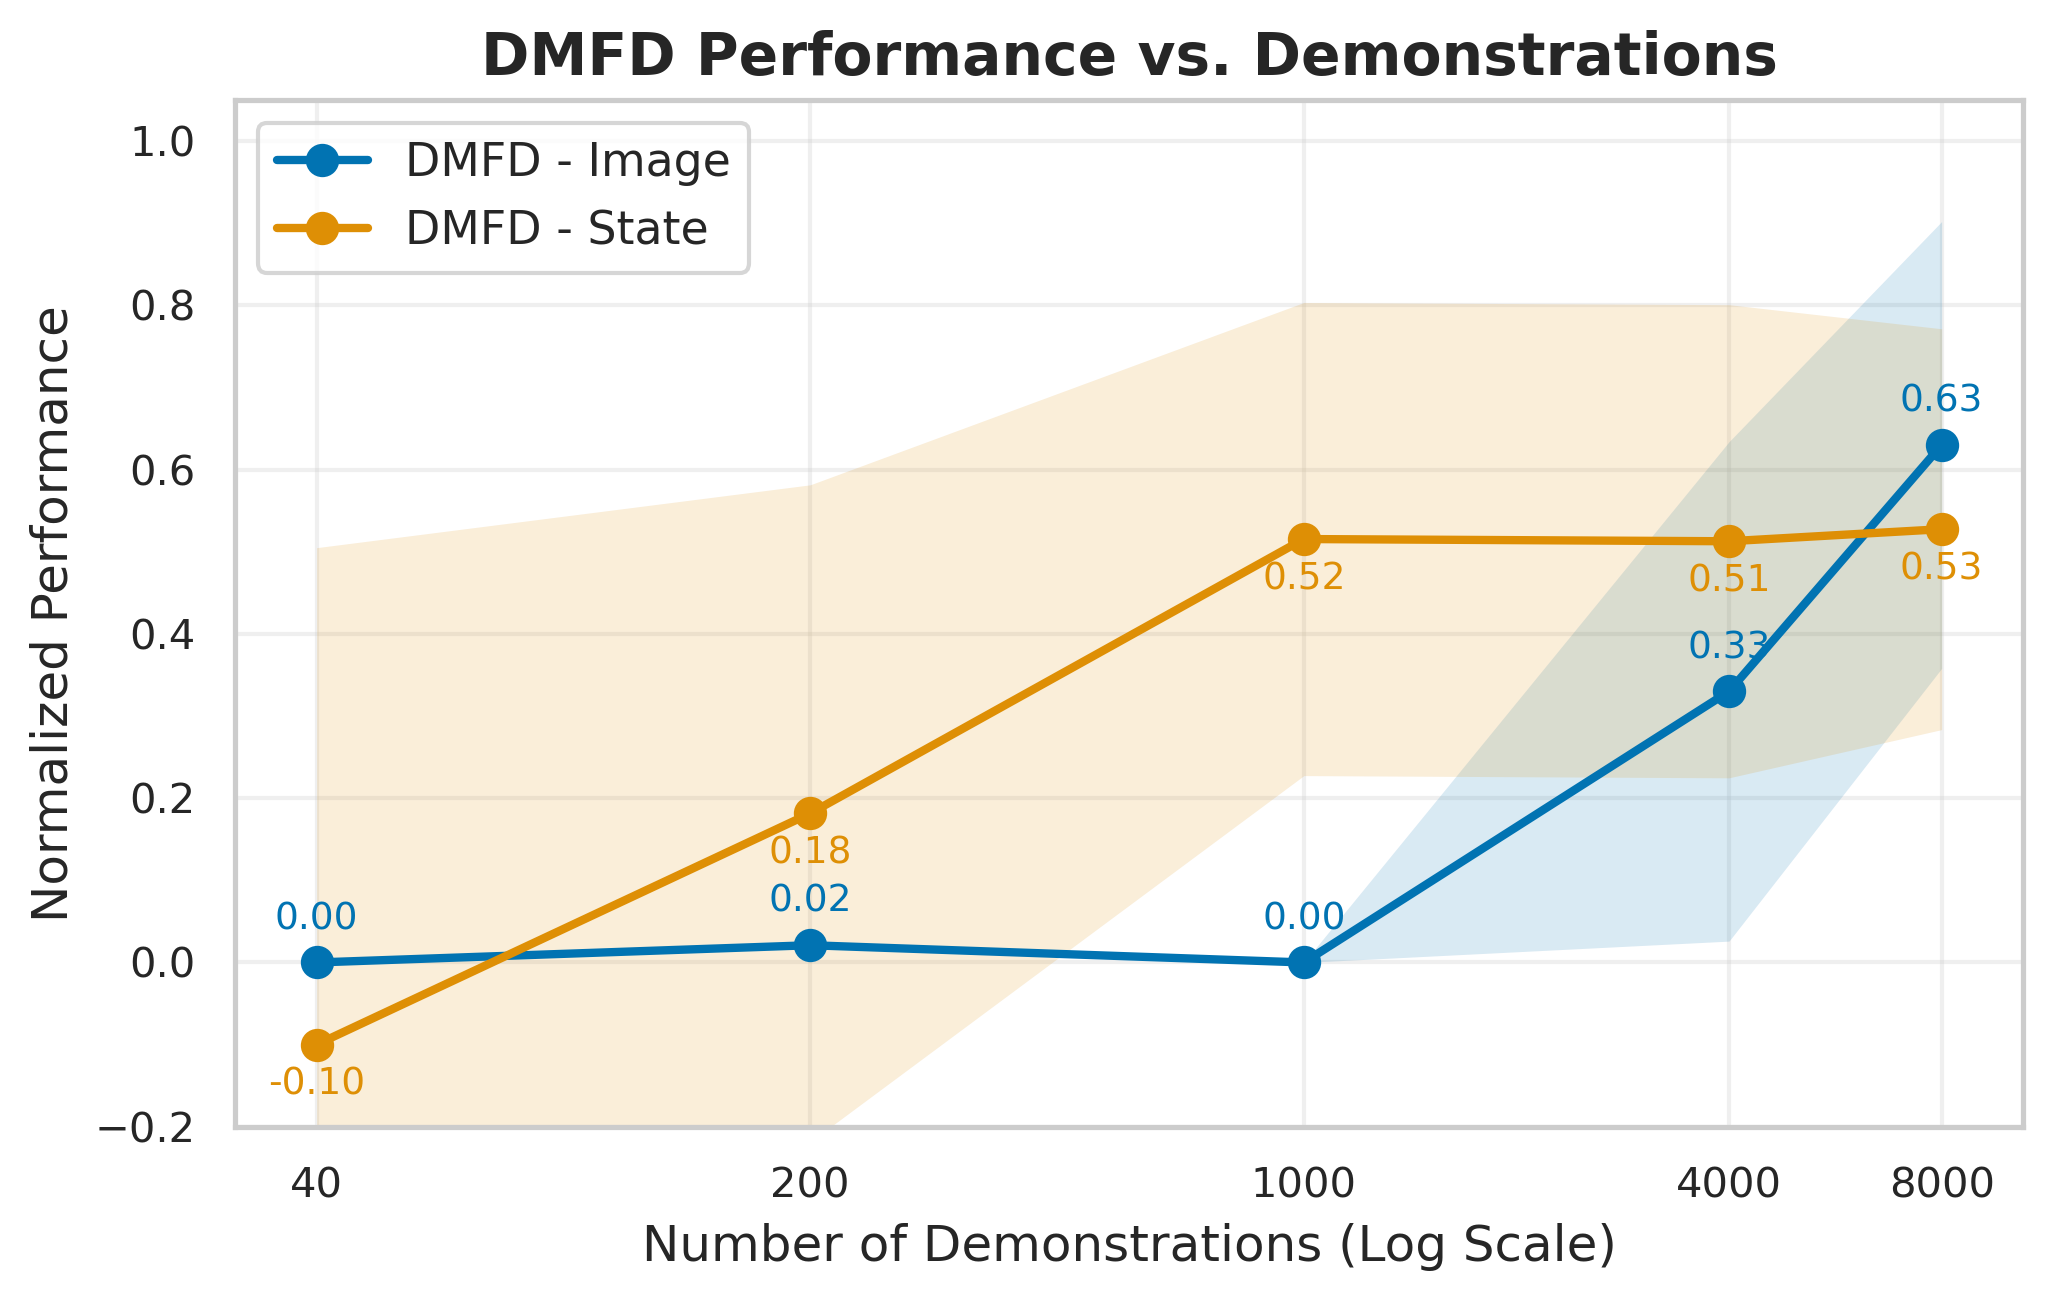
\includegraphics[width=0.49\textwidth]{img/cloth_fold/dmfd_performance_vs_num_dems.png}
    \hfill
    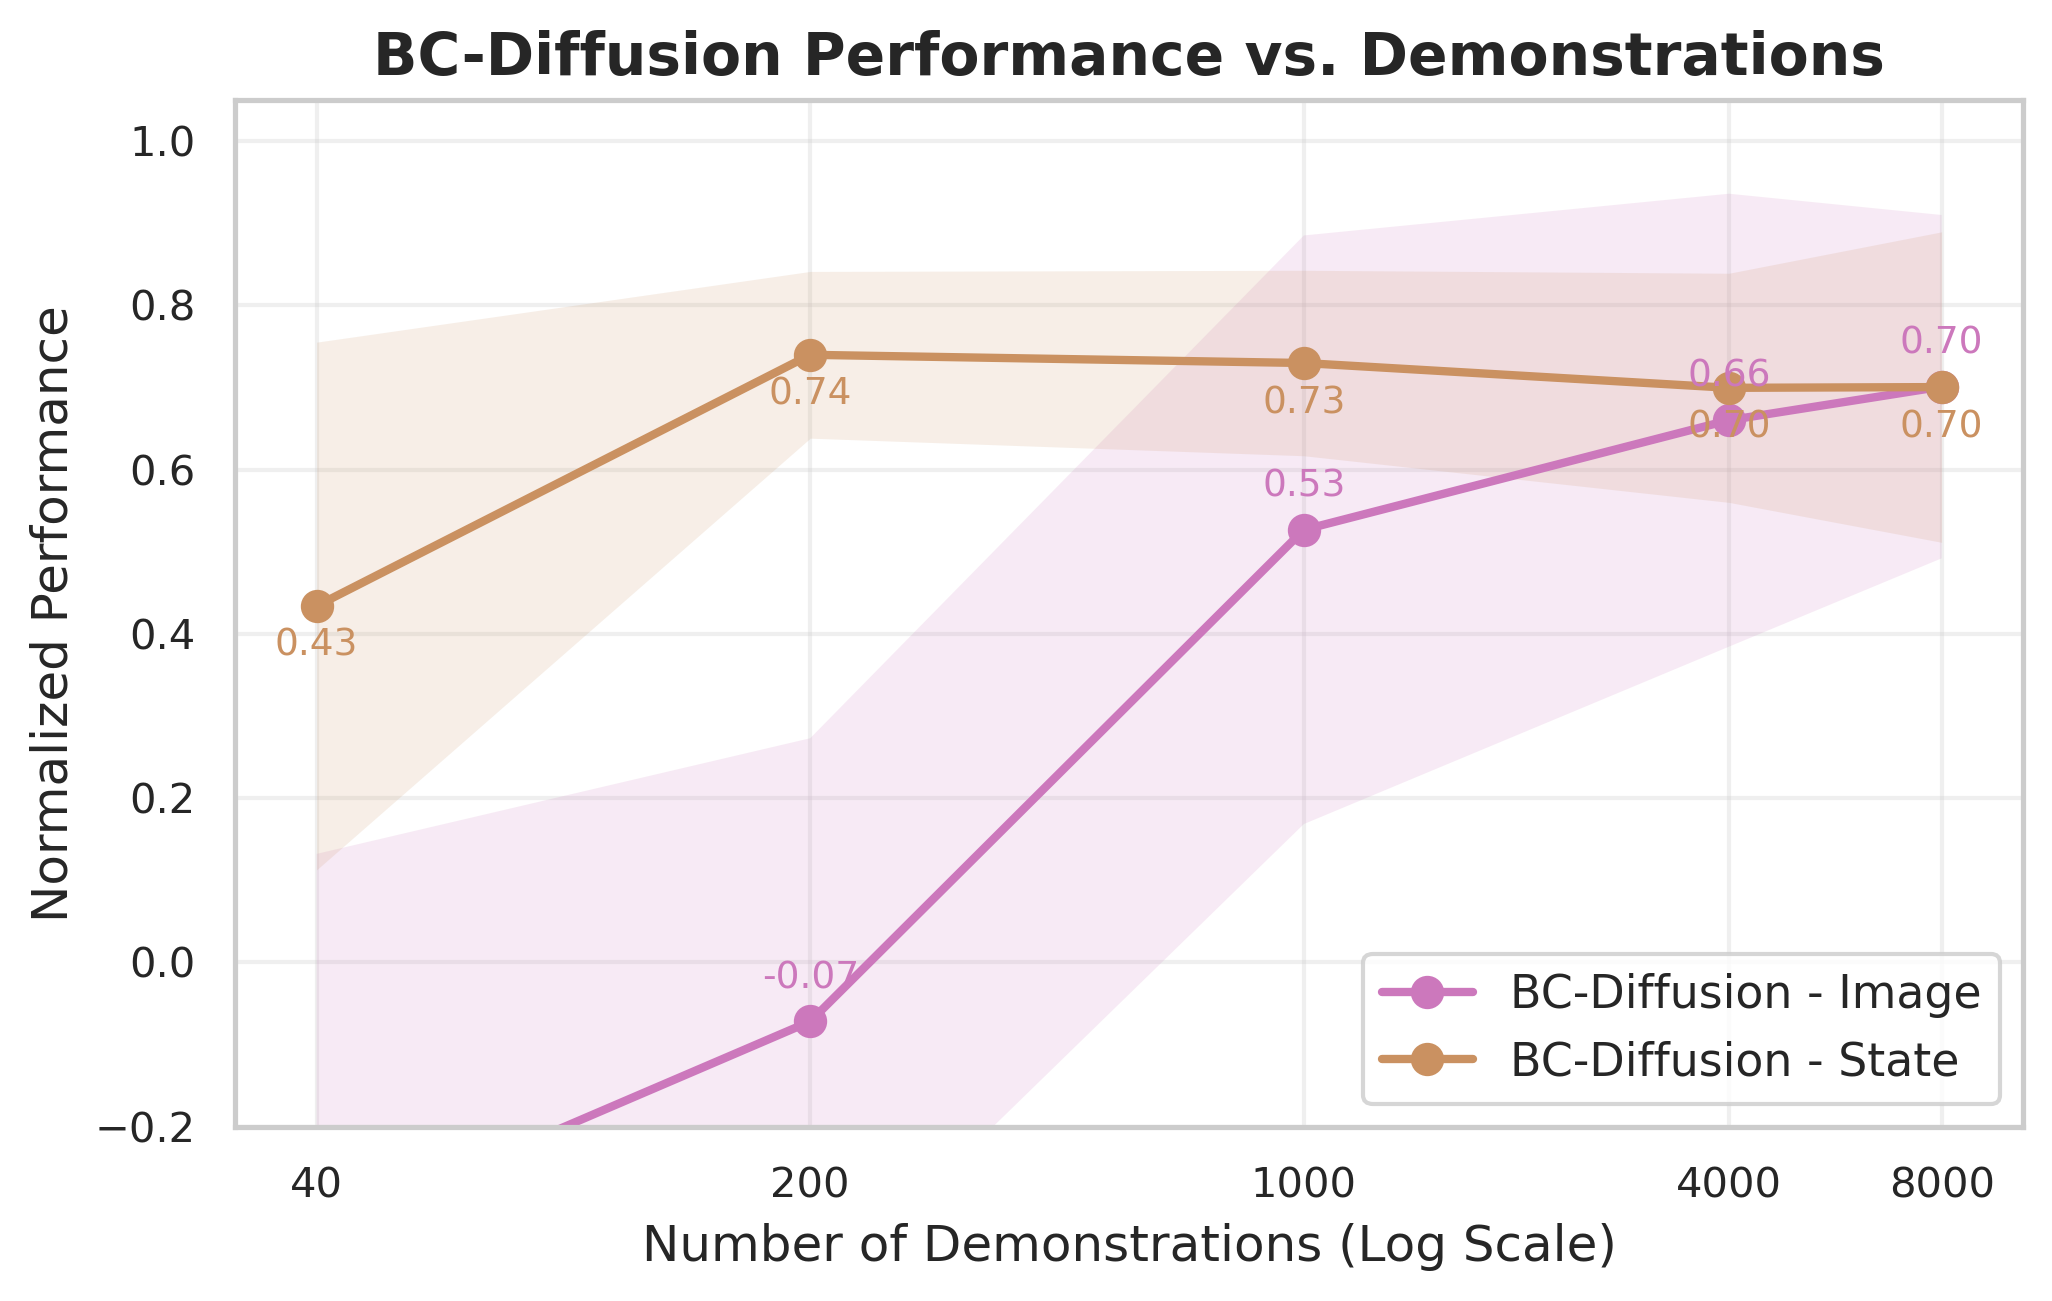
\includegraphics[width=0.49\textwidth]{img/cloth_fold/bc_diffusion_performance_vs_num_dems.png}
    \caption{
        Evaluation results for the Cloth Folding task. The plot shows the Normalized Performance (\(P_{\text{norm}}\), defined in Equation~\eqref{eq:norm_performance}, y-axis, higher is better) against the number of training demonstrations (logarithmic x-axis). Training data uses an 8:1 ratio of demonstrations to variations. Variations include random cloth sizes, initial rotations (\(\pm\pi/4\) radians), and subtle positional differences from cloth settling, promoting robust policies. Shaded regions indicate standard deviation. Each data point represents statistics from 100 evaluation episodes (20 episodes across 5 distinct random seeds) using deterministic actions from the agent model at end of training.
    }
    \label{fig:performance_vs_dems} % Label for cross-referencing
\end{figure}

\end{document}
